\documentclass{article}
\usepackage{amsmath}
\usepackage{amsfonts}
\usepackage{amssymb}
\usepackage{graphicx}
\usepackage{enumitem}
\usepackage{amsfonts}
\usepackage{amssymb}
\usepackage{xparse}
\usepackage{ifthen}
\usepackage{geometry}


\oddsidemargin=0in
\evensidemargin=0in
\textwidth=6in
\topmargin=0in
\textheight=9in

\parindent=0in
\pagestyle{empty}

\newcounter{EnumPrefix}
\newcounter{EnumSuffix}
%\newenvironment{Enum}[0]{
\DeclareDocumentEnvironment{Enum}{o}{
	\ifthenelse{ \equal{#1}{resume} }{
		\begin{enumerate}[label={\footnotesize\arabic{EnumPrefix}}.\arabic*]
		\setcounter{enumi}{\value{EnumSuffix}}
	}{
		\stepcounter{EnumPrefix}\begin{enumerate}[label={\footnotesize\arabic{EnumPrefix}}.\arabic*]
	}
}{
	\setcounter{EnumSuffix}{\value{enumi}}
	\end{enumerate}
}
%\renewcommand{\labelenumi}{\arabic{EnumPrefix}.\arabic*}

\newcommand{\ul}{$\underline{\phantom{xxx}}$}
\newcommand{\ull}{\underline{\phantom{xxx}}}
\newcommand{\xh}{\hat{\bf x}}
\newcommand{\yh}{\hat{\bf y}}
\newcommand{\zh}{\hat{\bf z}}
\newcommand{\R}{\mathbb{R}}
\newcommand{\C}{\mathbb{C}}
\newcommand{\Z}{\mathbb{Z}}
\newcommand{\N}{\mathbb{N}}
\newcommand{\proj}{\mathrm{proj}}
\newcommand{\mat}[1]{\begin{bmatrix}#1\end{bmatrix}}


\begin{document}
	\newgeometry{top=1cm}
	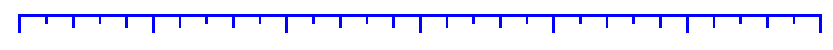
\includegraphics{ruler.pdf}
\section*{Vectors}

	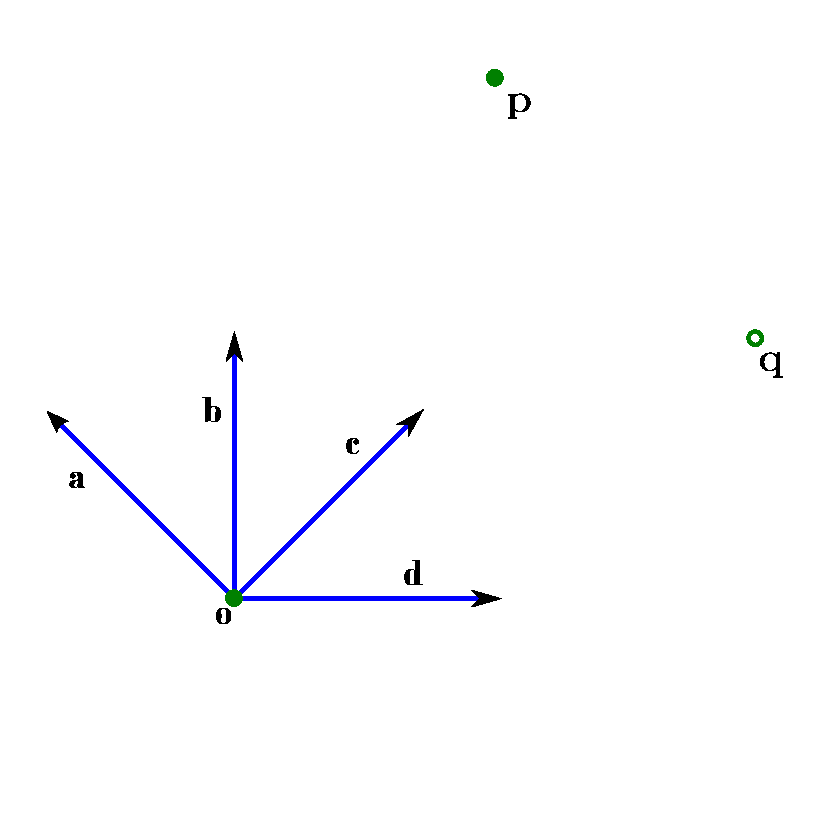
\includegraphics{vectors-graphically.pdf}

	Notice that all arrows in this diagram are the same length.
	We will call this length a \emph{unit}.
	\begin{Enum}
		\item Give directions from $\bf o$ to $\bf p$ of
		the form ``Walk \ul units in the direction of arrow \ul, then 
		walk \ul units in the direction of arrow \ul.''

		\item Can you give directions with the two arrows you haven't
		used?  Give such directions, or explain why it cannot be done.

		\item Give directions from $\bf o$ to $q$.

		\item Can you give directions from $\bf o$ to $q$ using $\bf c$ and $\bf a$?
		Give such directions, or explain why it cannot be done.

	\end{Enum}

\section*{Unit Vectors}
	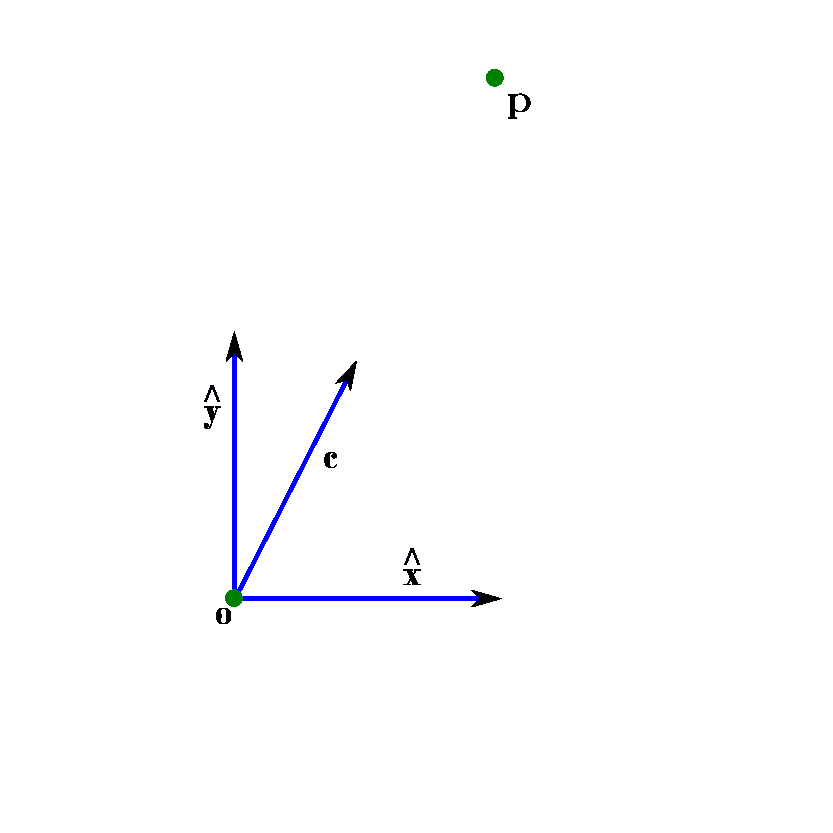
\includegraphics{vectors-graphically-2.pdf}

	We are going to start using a more mathematical notation
	for giving directions.  Our directions will now look like
	\[
		p = \ull\, \xh + \ull\, \yh
	\]
	which is read as ``To get to $p$ (=) go \ul units in the direction $\xh$ then (+) go \ul units in 
	the direction $\yh$.''

	\begin{Enum}
		\item What is the difference between $p = \ull\, \xh + \ull\, \yh$ and $p = \ull\, \yh + \ull\, \xh$?
		Can they both give valid directions?
		\item
		\begin{enumerate}
			\item Give directions to $p$ using the new notation. 
			\item Give directions to $p$ using $\bf c$.
			\item What is the distance from $\bf o$ to $p$ in units?
		\end{enumerate}
		\item
		\begin{enumerate}
			\item $r=1\bf c$.  Give directions from $\bf o$ to $r$ using $\xh$ and $\yh$.
			\item What is the distance from $\bf o$ to $r$?
		\end{enumerate}
		\item
		\begin{enumerate}
			\item $q=-2\xh+3\yh$; find the exact distance from $\bf o$ to $q$.
			\item $s=2\xh+\bf c$; find the exact distance from $\bf o$ to $s$.
		\end{enumerate}
	\end{Enum}

	We've been learning vector addition. $\xh$ and $\yh$ are called the \emph{standard
	basis vectors} for $\R^2$ (the plane).  Everyone has agreed that if we give directions
	from the origin to some point and we don't specify otherwise, we will give directions
	in terms of $\xh$ and $\yh$.

\section*{Column Vector Notation}
	We previously wrote $q=-2\xh+3\yh$.  In column vector notation we write
	\[
		q=\begin{bmatrix}-2\\3\end{bmatrix}
	\]
	We may call $q$ either a \emph{vector} or a \emph{point}.  If we call $q$ a vector,
	we are emphasizing that $q$ gives direction of some sort.  If we call $q$ a point,
	we emphasize that $q$ is some absolute location in space. (What's the philosophical
	difference between a location in space and directions from the origin to said location?)

	$r=1\bf c$; $s=2\xh+\bf c$.
	\begin{Enum}
		\item Write $r$ and $s$ in column vector form.
	\end{Enum}

\section*{Vector Length}
	The \emph{length} or \emph{norm} of a vector $\vec w$ is denoted $\|\vec w\|$ and is the distance
	from $\bf o$ to the point you end up at if you follow $\vec w$'s instructions.

	\begin{Enum}
		\item Find $\|\vec a\|$, $\|\vec b\|$, $\|\vec c\|$ where
		\begin{enumerate}
			\item $\vec a=3\xh+4\yh$
			\item $\vec b=2\vec a$
			\item $\vec c = -\vec a/2$
		\end{enumerate}
		\item $\zh$ points perpendicular to $\xh$ and $\yh$ into the 3rd dimension.
		
		Let $\vec v=2\xh+\yh+\zh$ and $\vec w=2\xh+\yh$.
		\begin{enumerate}
			\item Write $\vec v$ in terms of $\vec w$ and $\zh$
			and draw a picture showing the relationship between the three vectors
			(3-d pictures are a hard but essential skill in this course).
			\item Find $\|\vec w\|$ and $\|\vec v\|$.  (Hint, look at your picture
			and see if there are any right triangles to exploit).
		\end{enumerate}
		\item Let $\vec u=2\xh+3\yh+4\zh$.
		\begin{enumerate}
			\item Find $\|\vec u\|$.
			\item Find $\|k\vec u\|$ where $k$ is some unknown constant.
			\item What value(s) of $k$ makes $\|k\vec u\|=1$?
			\item Write down a vector in column form that points in the same direciton
			as $\vec u$ and has length 1.
		\end{enumerate}
	\end{Enum}

\section*{Unit Vectors}
	Vectors that have length 1 are called \emph{unit vectors}.
	\begin{Enum}
		\item $\vec a=-\xh+\yh+\zh$.  Find a unit vector in the direction of $\vec a$,
		and call this vector $\vec u$ ($u$ for $u$nit, get it?).
		\item Write $\vec a$ in terms of $\vec u$.  Does $\|\vec a\|$ show up in your formula at all?
		\item Write $3\vec u$ in column vector form and find its length.
		\item Write $7.5\vec u$ in column vector form and find its length.
		\item $\vec v$ is a different unit vector (I won't tell you its exact form).  Find $\|9\vec v\|$
		Why do we like unit vectors so much?
	\end{Enum}

\section*{Dot Product}
	The \emph{dot product} is incredible because it is easy to compute and has a useful
	geometric meaning.

	If $\vec a=\begin{bmatrix}a_1\\ a_2\\ \vdots \\ a_n\end{bmatrix}$ and 
	$\vec b=\begin{bmatrix}b_1\\ b_2\\ \vdots \\ b_n\end{bmatrix}$ are two vectors in $n$-dimensional
	space, then the dot product of $\vec a$ an $\vec b$ is
	\[
		\vec a\cdot\vec b = a_1b_1+a_2b_2+\cdots+a_nb_n.
	\]
	We also have a geometry-related formula
	\[
		\vec a\cdot \vec b = \|\vec a\|\|\vec b\|\cos \theta
	\]
	where $\theta$ is the angle between $\vec a$ and $\vec b$.
	
	\begin{Enum}
		\item Let $\vec a=\begin{bmatrix}1\\1\end{bmatrix}$ and $\vec b=\begin{bmatrix}3\\2\end{bmatrix}$
		\begin{enumerate}	
			\item Draw a picture of $\vec a $ and $\vec b$.
			\item Compute $\vec a\cdot \vec b$.
			\item Find $\|\vec a\|$ and $\|\vec b\|$ and use your knowledge of
			the multiple ways to compute the dot product to find $\theta$,
			the angle between $\vec a$ and $\vec b$. Label $\theta$ on your picture.
		\end{enumerate}
		\item Draw the graph of $\cos$ and identify which angles make $\cos$ negative, zero,
		or positive.

		\item Draw a new picture of $\vec a$ and $\vec b$ and on that picture draw
		\begin{enumerate}	
			\item a vector $\vec c$ where $\vec c\cdot \vec a$ is negative.
			\item a vector $\vec d$ where $\vec d\cdot \vec a=0$ and $\vec d\cdot \vec b < 0$.
			\item a vector $\vec e$ where $\vec e\cdot \vec a=0$ and $\vec e\cdot \vec b>0$.
			\item Could you find a vector $\vec f$ where $\vec f\cdot \vec a=0$ and $\vec f\cdot \vec b=0$?
			Explain why or why not.
		\end{enumerate}

		\item $\vec u=\begin{bmatrix}1\\2\\1\end{bmatrix}$.
		\begin{enumerate}
			\item Write down a vector $\vec v$ so that the angle between $\vec u$ and $\vec v$
			is $\pi/2$. (Hint, how does this relate to the dot product?)
			\item Write down another vector $\vec w$ (in a different direction from $\vec v$)
			so that the angle between $\vec w$ and $\vec u$ is $\pi/2$.
			\item Can you write down other vectors different than both $\vec v$ and $\vec w$ that still
			form an angle of $\pi/2$ with $\vec u$?  How many such vectors are there?
		\end{enumerate}
	\end{Enum}

	We've explored how dot products relate to angles, but how do they relate to lengths?
	\begin{Enum}
		\item Let $\vec a = \begin{bmatrix}3\\3\\-1\end{bmatrix}$
		\begin{enumerate}
			\item Find $\|\vec a\|$ and $\vec a\cdot \vec a$.  How do the
			two quantities relate?
			\item Write down an equation for the length of a vector $\vec v$ in terms
			of dot products.
		\end{enumerate}
		\item Let $\vec b = \begin{bmatrix}1\\1\\-2\\2\end{bmatrix}$, and find $\|\vec b\|$.
		Did you know how to find 4-d lengths before?
		\item Suppose $\vec u=\begin{bmatrix}x\\ y\end{bmatrix}$ for $x,y\in \R$.
		Could $\vec u\cdot \vec u$ be negative? Compute $\vec u\cdot \vec u$ algebraically
		and use this to justify your answer.
	\end{Enum}

\section*{Projections}
	Projections (sometimes called orthogonal projections) are a way to measure how much one vector
	points in the direction of another.

	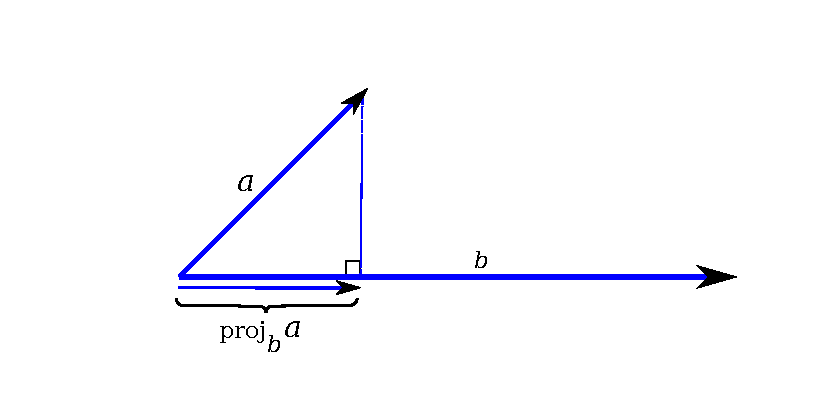
\includegraphics{projection1.pdf}

	The projection of $\vec a$ onto $\vec b$ is written $\proj_{\vec b}\vec a$ and is a vector in the direction of $\vec b$.

	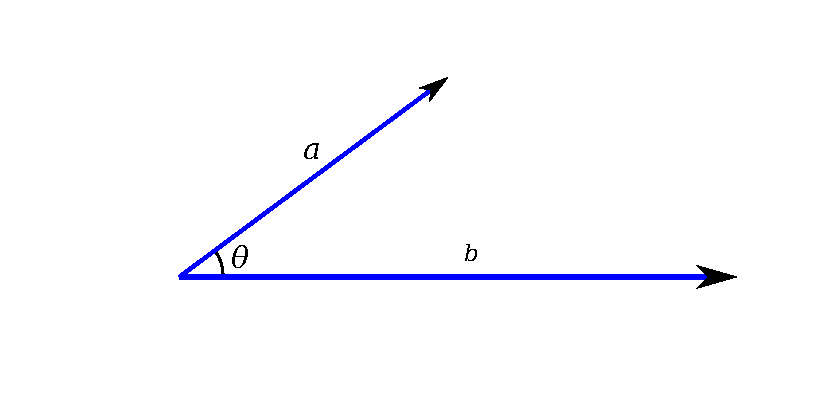
\includegraphics{projection2.pdf}
	
	\begin{Enum}
		\item In this picture $\|\vec a\|=4$ and $\theta = \pi/6$.  Find $\|\proj_{\vec b}\vec a\|$.
		\item If $\vec b=\begin{bmatrix}6\\0\end{bmatrix}$, write down $\proj_{\vec b}\vec a$ in column vector
		form.  How do the coordinates relate to $\|\proj_{\vec b}\vec a\|$?
		\item Consider $\vec u=\begin{bmatrix}3\\1\end{bmatrix}$.  Compute $\proj_{\xh}\vec u$ and 
		$\proj_{\yh}\vec u$.  How do these projections relate to the coordinates of $\vec u$? What
		can you say in general about projections onto $\xh$ and $\yh$?
	\end{Enum}

	\[
		\vec w = \begin{bmatrix}4\\4\end{bmatrix}\qquad \vec v=\begin{bmatrix}2\\7\end{bmatrix}
	\]
	\begin{Enum}
		\item Find $\theta$, the angle between $\vec w$ and $\vec v$.
		\item Use $\theta$ to compute $\proj_{\vec v}\vec w$ and $\proj_{\vec w}\vec v$.
		\item Write down a formula for $\proj_{\vec b}\vec a$ where $\vec a$ and $\vec b$ are
		arbitrary vectors.
	\end{Enum}
	\begin{Enum}
		\item For the arbitrary vector $\vec a$, what is $\proj_{3\vec a}\vec a$?
		\item If $\vec a$ and $\vec b$ are orthogonal (perpendicular) vectors,
		what is $\proj_{\vec b}\vec a$ $\proj_{\vec a}\vec b$?
	\end{Enum}
	

\section*{Lines, Planes, Normals, Equations}
	\begin{Enum}
		\item Draw $\vec u=\begin{bmatrix}2\\3\end{bmatrix}$ and \emph{all}
		vectors perpendicular to it.
		\item If $\vec x=\begin{bmatrix}x\\y\end{bmatrix}$ and $\vec x$ is 
		perpendicular to $\vec u$, what is $\vec x\cdot \vec u$?
		\item Expand the dot product $\vec u\cdot \vec x$ to get an equation
		for a line.  This is called \emph{normal form}
	\end{Enum}

	A \emph{normal vector} to a line is one that is orthogonal to it.
	\begin{Enum}[resume]
		\item Rewrite the line $\vec u\cdot \vec x = 0$ in $y=mx+b$ form and verify it matches
		the line you drew above.
	\end{Enum}

	We can also write a line in \emph{parametric form} by introducing a parameter
	that traces out the line as the parameter runs over all real numbers.
	\begin{Enum}
		\item Draw the line $L$ with $x,y$ coordinates given by
		\[
			\begin{array}{l}x=t\\y=2t\end{array}
		\]
		as $t$ ranges over $\R$.
		\item Write the line $\vec u \cdot \vec x=0$ (where $\vec u$ is the same as before) in parametric form.
	\end{Enum}
	
	\emph{Vector form} is the same as parametric form but written in vector notation.  For example, the
	line $L$ from earlier could be written as 
	\[
		\begin{bmatrix}x\\y\end{bmatrix}=\begin{bmatrix}t\\2t\end{bmatrix}
	\]
	or
	\[
		\begin{bmatrix}x\\y\end{bmatrix}=t\begin{bmatrix}1\\2\end{bmatrix}.
	\]

	\begin{Enum}
		\item Write $\vec u\cdot \vec x=0$ in vector form.  That is, find a vector $\vec v$ so
		the line $\vec u\cdot \vec x=0$  can be written as
		\[
			\begin{bmatrix}x\\y\end{bmatrix} = t\vec v
		\]
		as $t$ ranges over $\R$.
		\item What is $\vec v\cdot \vec u$? Why? Will this always happen?
	\end{Enum}

	\subsection*{Moving to Planes}
	When solving equations, sometimes we get to make choices. For example, 
	if $x+2y=0$, we can find solutions by fixing either $x$ or $y$ and solving
	for the other. e.g., if $x=2$, then $y=-1$ nad if $y=3$ then $x=-6$.

	\begin{Enum}
		\item Write down three solutions $\vec a$, $\vec b$, $\vec c$ to
		\begin{equation}\label{eq1}
			2x+y-z=0.
		\end{equation}
		\item Is $2\vec a-\vec b$ a solution?  Is any linear combination of solutions a solution?  Justify why or why not.
		\item Rewrite equation (\ref{eq1}) in normal form $\vec n\cdot \vec x=0$ where $\vec x=\begin{bmatrix}x\\ y\\ z\end{bmatrix}$.
		\item What do you notice about the angle between solutions to equation (\ref{eq1}) and $\vec n$?
		\item You've already seen that scalars come out of dot products (e.g., $\vec a\cdot(3\vec b) = 3(\vec a\cdot \vec b)$.
		Use this combined with normal form to prove a linear combination of solutions is still a solution.
	\end{Enum}

	When writing down solutions to equation (\ref{eq1}), you got to choose two coordinates before the remaining
	coordinate became determined.  This means the solutions have two parameters (and consequently form a
	two dimensional space).

	\begin{Enum}[resume]
		\item Write down parametric form of a line of solutions to equation (\ref{eq1}).
		\item Write down parametric form of a different line of solutions to equation (\ref{eq1}).
		\item Write down all solutions to equation (\ref{eq1}) in parametric form.  That is, find $a_x,
		a_y,a_z,b_x,b_y,b_z$ so that
		\[
			\begin{array}{l}
				x=a_x t+b_x s\\
				y=a_y t+b_y s\\
				z=a_z t+b_z s
			\end{array}
		\]
		gives all solutions as $t,s$ vary over all of $\R$.
		\item Write all solutions to equation (\ref{eq1}) in vector form.
	\end{Enum}

\subsection*{Arbitrary Lines and Planes}
	
	So far, all of our lines and planes have passed through the origin. To 
	produce the equation of an arbitrary line/plane, we first make one of
	same ``slope'' that passes through the origin, then we translate it
	to the appropriate place.

	We'd like to write the equation of a line $L$ with normal vector
	$\vec n=\begin{bmatrix}4\\-1\end{bmatrix}$ that passes through
	the point $p=\mat{-1\\-1}$

	\begin{Enum}
		\item Write normal form of the line $L_2$ which is parallel to $L$,
		but passes through the origin.
		\item Draw a picture of $L$ and $L_2$, and find two points that lie on
		$L$.  Call these points $p_1$ and $p_2$.
		\item Verify the vector $\vec {p_1p_2}$ is perpendicular to $\vec n$.
		\item What is $\vec n\cdot p_1$, $\vec n\cdot p_2$, $\vec n\cdot p$?
		Should these values be zero, equal, or different?  Explain (think about
		projections).
		\item How does the equation $\vec n\cdot (\vec x-p)=0$ relate to $L$?
	\end{Enum}

	$W$ is the plane with normal vector $\vec n=\mat{1\\2\\3}$ and passes through
	the point $p=\mat{1\\1\\2}$.
	\begin{Enum}
		\item Write normal form of $W$.
		\item Write vector form of $W$.
	\end{Enum}

\section*{Systems of Linear Equations}
	
	\emph{Linear equations} are equations only involving variables, 
	multiplication by constants, and addition/subtraction.  \emph{Systems}
	of equations are sets of equations that share common variables.

	Consider the system
	\begin{equation}\label{eq2}
		\begin{array}{ll}
			x-y &= 2\\
			2x+y &= 1
		\end{array}
	\end{equation}

	\begin{Enum}
		\item Draw the lines in (\ref{eq2}) on the same coordinate plane.
		\item Algebraically solve the system (\ref{eq2}).  What does this 
		solution represent on your graph?
	\end{Enum}
	Let $L$ be the line given by $x-y=2$.
	\begin{Enum}
		\item Write an equation of a line that doesn't intersect $L$.
		\item Write an equation of a line that intersects $L$ in 
		\begin{enumerate}
			\item one place.
			\item infinitely many places
			\item exactly two places
		\end{enumerate}
		or explain why no such equation exists.
		\item For each equation you came up with solve the system algebraically.
		How can you tell algebraically how many solutions there are?
	\end{Enum}

\subsection*{The Row Reduction Algorithm}

	\begin{Enum}
		\item Solve the system
		\begin{equation}\label{eq3}
			\begin{array}{ll}
				x-y-2z &= -5\\
				2x+3y+z &= 5\\
				0x+2y+3z &= 8
			\end{array}
		\end{equation}
		any way you like.

		\item Use an augmented matrix to solve the system (\ref{eq3}).
	\end{Enum}

	The system (\ref{eq3}) can be interpreted in two ways (and switching between these 
	interpretations when appropriate is one of the most powerful tools of Linear 
	Algebra).  We can think of solutions to (\ref{eq3})
	as the intersection of three planes, or we can interpret the solution
	as coefficients of a linear combination.

	\begin{Enum}[resume]
		\item Rewrite (\ref{eq3}) as a vector equation of the form
		\[
			x\vec v_1+y\vec v_2+z\vec v_3 = \vec p
		\]
		where $x,y,z$ are interpreted as scalar quantities.

		\item If $(x,y,z)$ is a solution to (\ref{eq3}), explain how to get from the
		origin to $\vec p$ using only $\vec v_1, \vec v_2, \vec v_3$.
	\end{Enum}



\end{document}
